%
% File emnlp2020.tex
%
%% Based on the style files for ACL 2020, which were
%% Based on the style files for ACL 2018, NAACL 2018/19, which were
%% Based on the style files for ACL-2015, with some improvements
%%  taken from the NAACL-2016 style
%% Based on the style files for ACL-2014, which were, in turn,
%% based on ACL-2013, ACL-2012, ACL-2011, ACL-2010, ACL-IJCNLP-2009,
%% EACL-2009, IJCNLP-2008...
%% Based on the style files for EACL 2006 by
%%e.agirre@ehu.es or Sergi.Balari@uab.es
%% and that of ACL 08 by Joakim Nivre and Noah Smith

\documentclass[11pt,a4paper]{article}
\usepackage[hyperref]{emnlp2020}
\usepackage{times}
\usepackage{latexsym}

\usepackage{url}
\usepackage{booktabs}
\usepackage{graphicx}
\usepackage{blindtext}
\usepackage[autostyle=true]{csquotes}



\renewcommand{\UrlFont}{\ttfamily\small}

% This is not strictly necessary, and may be commented out,
% but it will improve the layout of the manuscript,
% and will typically save some space.
\usepackage{microtype}

%\aclfinalcopy % Uncomment this line for the final submission
%\def\aclpaperid{***} %  Enter the acl Paper ID here

%\setlength\titlebox{5cm}
% You can expand the titlebox if you need extra space
% to show all the authors. Please do not make the titlebox
% smaller than 5cm (the original size); we will check this
% in the camera-ready version and ask you to change it back.

\newcommand\BibTeX{B\textsc{ib}\TeX}

\title{Diversity, Pragmatic Informativeness and Semantic Adequacy in Character-Level Image Captioning: A Comparison of Decoding Strategies}

\author{First Author \\
  Affiliation / Address line 1 \\
  Affiliation / Address line 2 \\
  Affiliation / Address line 3 \\
  \texttt{email@domain} \\\And
  Second Author \\
  Affiliation / Address line 1 \\
  Affiliation / Address line 2 \\
  Affiliation / Address line 3 \\
  \texttt{email@domain} \\}

\date{}

\begin{document}
\maketitle

% Abstract

\begin{abstract}
%\blindtext
\end{abstract}

% Text

\section{Introduction}

% maybe a bit more detail on different requirements for decoding strategies, depending on the task (open-ended vs. directed generation \citep{holtzman-etal-2018-learning}
% disclaimer: no state-of-the-art results; focus on comparing the different decoding strategies, speaker/listener setup needed for pragmatic evaluation

Neural models with encoder-decoder architectures and RNN-based sequence generation are used for a variety of problems in Language and Vision (L\&V), e.g. Image Captioning or Referring Expression Generation. 

So far, research has mainly focused on the training of the models \citep{zarriess-schlangen-2018-decoding}.
L\&V models are most commonly optimized to generate human-like descriptions for a given image: During training this is reflected by the usage of Maximum Likelihood Estimation objectives, in evaluation by aiming for the best possible results in metrics such as BLEU \citep{papineni-etal-2002-bleu} and CIDER \citep{Vedantam2014}, which rely on the similarity to given ground-truth captions. 
More recently, however, the decoding process, i.e. the way in which word sequences can be derived from token probabilities for individual steps, has also received increasing attention.

A basic decoding strategy in sequence generation is to pick the token with the highest probability in each step until an end token is generated \textit{greedy search}. However, in many cases this method does not allow for optimal results and often leads to repetitive sentences or sentences that are defective in some other way. For this reasons it has been extended in different ways. 
A common extension is to simultaneously expand a defined number of hypotheses in each step (\textit{beam search}). While this often leads to improved results regarding metrics like BLEU or CIDEr, other issues with greedy decoding are not solved: Beam Search often leads to short and repetitive sentences which are very similar to each other and in which only a small part of the available vocabulary is used. 
These shortcomings are addressed by various attempts to enhance diversity through e.g. stochastic decoding strategies such as \textit{Top-K Random Sampling} \citep{fan-etal-2018-hierarchical} or \textit{Nucleus Sampling} \citep{Holtzman2019} (cf. \citet{Ippolito2019} for a comprehensive overview). There appears to be a trade-off between likelihood and diversity: Models which where shaped to provide sequences as similar as possible to human annotations were shown to produce a less diverse output. Models with a optimized diversity achieve lower results on metrics like BLEU or CIDEr \citep{Wang2019}.

While diversity enhancing decoding strategies are reported to be effective in terms of more diverse outputs, their linguistic implications are to be viewed critically. Both Nucleus Sampling and Top-K Random Sampling are based on randomness - the language model is used to determine a set of possible candidates, then the tokens to be generated are randomly selected from this set. The diversity of the resulting utterances can thus be seen as being caused by blurring the predictions of the trained model with respect to specific tokens. This seems appropriate for tasks such as conditional story generation, in which the stylistic properties of the generated text play an important role. 
Strictly speaking, however, this form of linguistic diversity can be seen as an illusion, since it does not reflect the creative and intentional use of language that underlies the diversity of human utterances. (pragmatic aspects of vocabulary choice: e.g. gricean maximes, as described by \citet{Cruse1977} \citep{reiter-1990-new}, \citep{Reiter1991})

Moreover, essential aspects of language are disregarded in Beam Search as well as in Nucleus Sampling or Top-K Random Sampling. In actual language use, linguistic utterances are not only true and well-formed, but also goal-oriented, as formulated, for example, by speech act theory or the Gricean Cooperative Principle. Even if the output of diversity-focused decoding strategies is more varied both structurally and lexically, it remains unclear whether this diversity is used purposefully by the model, for example to describe a visual referent as meaningfully as possible. This pragmatic informativity can be enhanced during decoding e.g. by using strategies built on the Rational Speech Acts (RSA) framework \citep{Cohn-Gordon2018}.

In this work, we want to explore the interactions between likelihood, diversity and pragmatic informativity. For this, we want to compare different decoding strategies that are focused on optimal results for these individual aspects. We want to compare Beam Search (which was shown to yield good results in likelihood-based evaluation metrics), Nucleus Sampling (which is designed to tackle the diversity issues that arise with Beam Search), and RSA-based greedy decoding (which is focused on improving discrimination between targets and competing distractors e.g. in REG-like tasks). We test these approaches by using evaluation metrics that reflect the agreement of the generated sentences with ground-truth annotations, the diversity of the resulting captions, or the pragmatic informativeness with which the referents are described in the context of similar distractors.

We hypothesize that neither the increased (lexical) diversity in utterances produced using Nucleus Sampling nor the likelihood to human utteranced of captions produced using Beam Search lead to a higher pragmatic informativeness as compared to a greedy decoding baseline. Conversely, we assume that the introduction of additional pragmatic constraints in the RSA-based decoding leads to increased diversity compared to both to Greedy and Beam Search.

\begin{itemize}

	\item research questions: 
	\begin{enumerate}
		\item how does pragmatic decoding relate to greedy, beam + nucleus? (does it increase/decrease scores on likelihood metrics? does it increase/decrease scores on diversity metrics?)
		\item are there structural differences (e.g. word types used) between the decoding strategies? (how does diversity look like if we look at it on a more detailed level?
		\item what are the differences between the decoding strategies if tested with a neural listener model?
		\item how do diversity enhancing decoding strategies work for character level decoding?
	\end{enumerate}

\end{itemize}

\section{Related Work}

\begin{itemize}
	\item pragmatics in image descriptions / captioning: \citet{Miltenburg2016}, \citet{Cohn-Gordon2018}
	\item decoding + diversity
	\citep{ippolito-etal-2019-comparison} \citep{Wang2019} \citep{van-miltenburg-etal-2018-measuring} structural properties of language \citep{ghodsi-denero-2016-analysis} \citep{Lippi2018}
	\begin{itemize}
		\item \citep{zarriess-schlangen-2018-decoding}
	\end{itemize}
	\item diversity
	\item reinforcement learning
	\item rational speech acts

\end{itemize}

\section{Models, Methods, Data}

\subsection{Model}

model description

\subsection{Decoding Strategies}

all decoding strategies: character level (because of RSA, other reasons?)
character level for rsa: if made on word level, it would require some kind of pruning in order to be computationally feasible \citep{Cohn-Gordon2018}. if we assess the lexical diversity, we should allow the model at least in theory to produce all words seen during the training

\paragraph{Greedy Decoding} We use a simple Greedy decoding algorithm as our baseline: At each tim step, the word with the highest probability is selected and appended to the output sequence. The algorithm terminates after the generation of the end token or when the maximal sequence length is reached \citep[cf. e.g.][]{zarriess-schlangen-2018-decoding}.
\paragraph{Beam Search} In Beam Search, a fixed number of hypotheses is kept and expanded simultaneously at each step \citep[cf. e.g.][]{Graves2012}. According to \citet{zarriess-schlangen-2018-decoding}, beam search algorithms can be modified in numerous ways, e.g. by specifying constant or dynamic values for the number of hypotheses considered at the same time (beam size), restricting possible next candidates (pruning), defining more sophisticated finishing conditions (termination) or normalizing candidates with different lengths. Here, we use a rather standard approach - we use static beam widths, refrain from pruning or length normalization, and terminate the beam search if the top candidate has the end token as its final segment.
\paragraph{Nucleus Decoding}

\begin{itemize}
	\item \enquote{In practice this means selecting the highest probability tokens whose cumulative probability massexceeds the pre-chosen thresholdp.  The size of the sampling set will adjust dynamically based onthe shape of the probability distribution at each time step. For high values ofp, this is a small subsetof vocabulary that takes up vast majority of the probability mass — the nucleus.} \citet{Holtzman2019}
\end{itemize}

\paragraph{Greedy RSA Decoding}

\begin{itemize}
	\item model implemeted as a \enquote{pragmatic speaker}: a RSA model is combined with the neural image captioning model to produce captions that distinguish targets from similar images
	\item rsa speaker reasons about how the produced captions would be understood by a listener, to assess whether the utterances produced are capable of distinguishing the target
	\item \citet{Cohn-Gordon2018}
	\item whereas \citet{Cohn-Gordon2018} report results for a beam search variant, we focus on a greedy search method. The reasons for that are 1) computational constraints (we use a much larger test set compared to the 100 images / image clusters in the original paper) and 2) that the comparison to captions generated using beam search is less concise if the decoding strategy itself is a kind of beam search. this way, we have beam search, nucleus sampling and rsa decoding as three greedy search extensions, which have a minimal overlap. 
	\item RSA approach used in REG \citep{zarriess-schlangen-2019-know} and other language generation tasks \citep{Shen2019}
\end{itemize}


\subsection{Evaluation Metrics}

\paragraph{Likelihood} BLEU / CIDEr
\paragraph{Diversity}
\paragraph{Pragmatic Informativity} a listener model reproduces captions produced by a speaker model in a greedy-like fashion, given a set of potential target images. for each token the model updates the probabilities for every image - the candidate with the highest probability is chosen as the target image. The accuracy and MRR of the choice of target images is compared between the decoding strategies.

\subsection{Data}

\begin{itemize}
	\item images and annotations from MSCOCO \citep{Lin2014}
	\item speaker and listener models each trained on one half of the train partition
	\item random sample of 5000 images from val partition used for testing
\end{itemize}


\section{Experiments}

\subsection{Likelihood and Diversity Tradeoffs}


\begin{itemize}

\item method
	\begin{itemize}
	\item assess BLEU and CIDEr scores for different decoding strategies and hyperparameters
	\item compare between each other and to greedy baseline
	\end{itemize}

\item goal
	\begin{itemize}
	\item determining whether likelihood \& diversity tradeoff holds for beam search vs. nucleus decoding and how RSA decoding performs in terms of likelihood and diversity
	\end{itemize}

\item results
	\begin{itemize}
	\item likelihood: beam search best, pragmatic worst. greedy > nucleus
	\item diversity: higher for pragmatic than for beam search / greedy (nucleus: depends on hyperparameters)
	\end{itemize}

\end{itemize}



%\begin{figure*} \centering 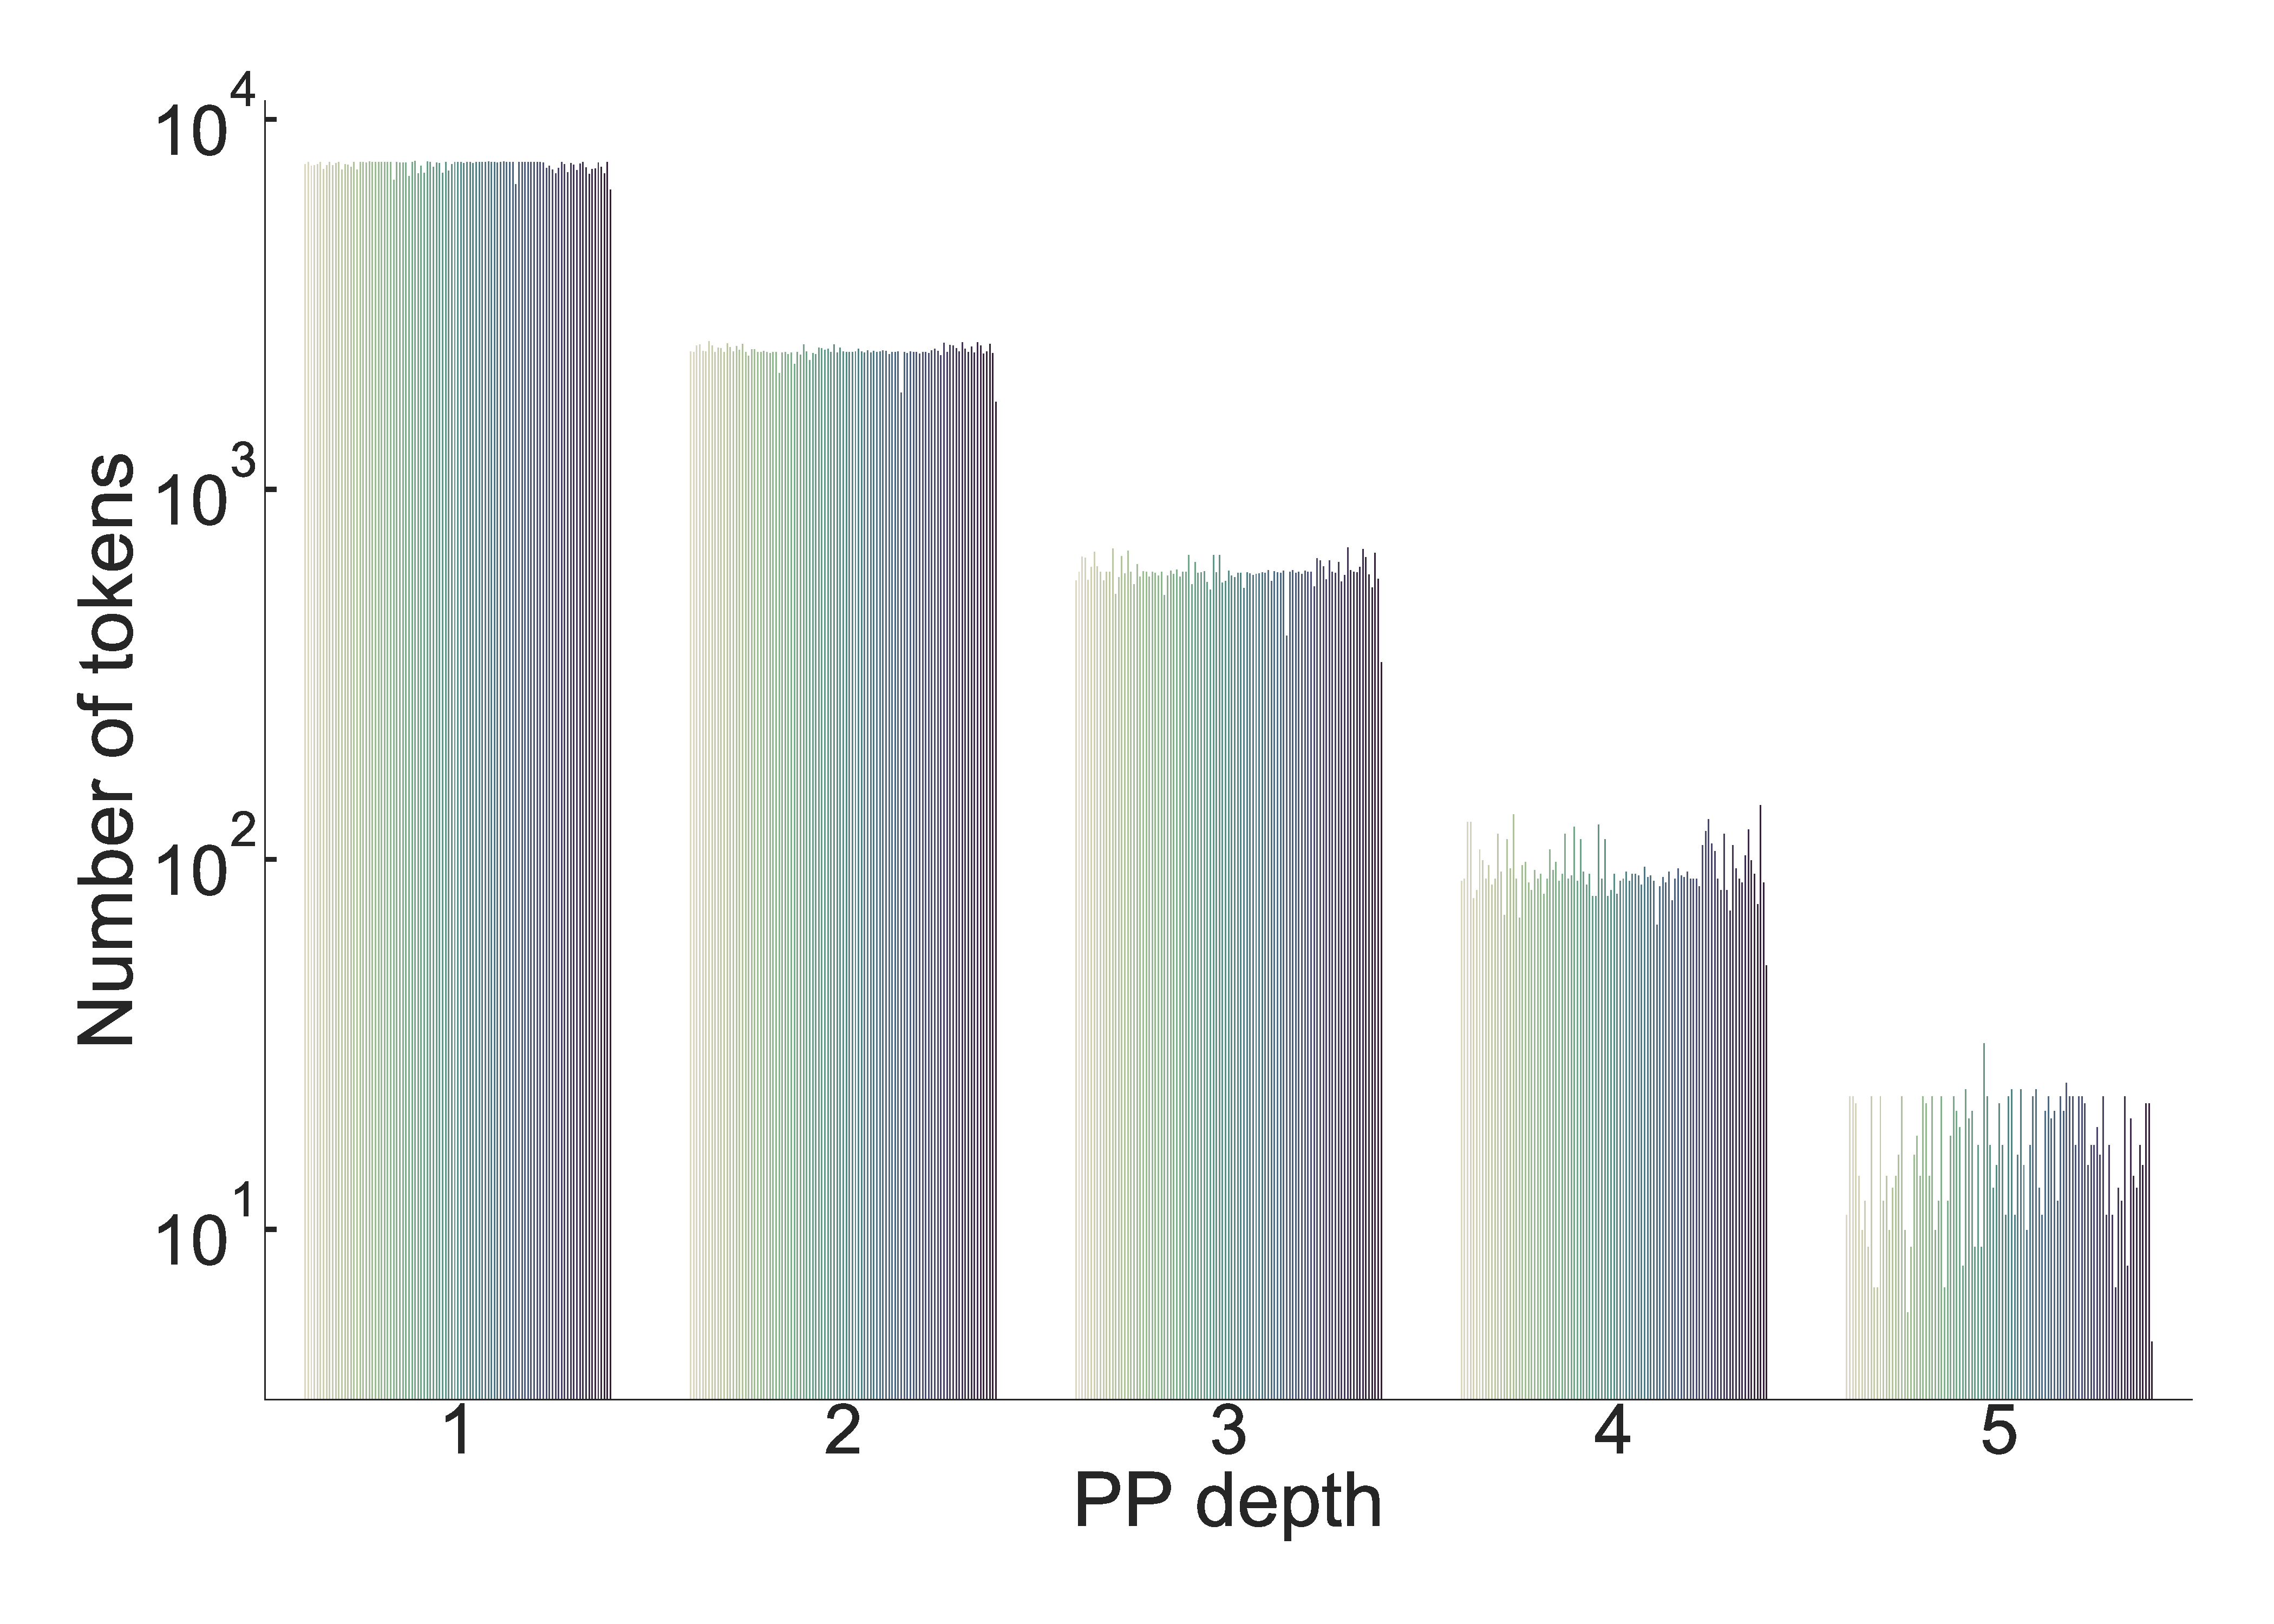
\includegraphics[width=\columnwidth]{figs/pp_depths.pdf} \end{figure*}

%\begin{figure*} \centering \includegraphics[width=\columnwidth]{figs/ttr_curve_nolegend.pdf} \end{figure*}

%\begin{figure*} \centering 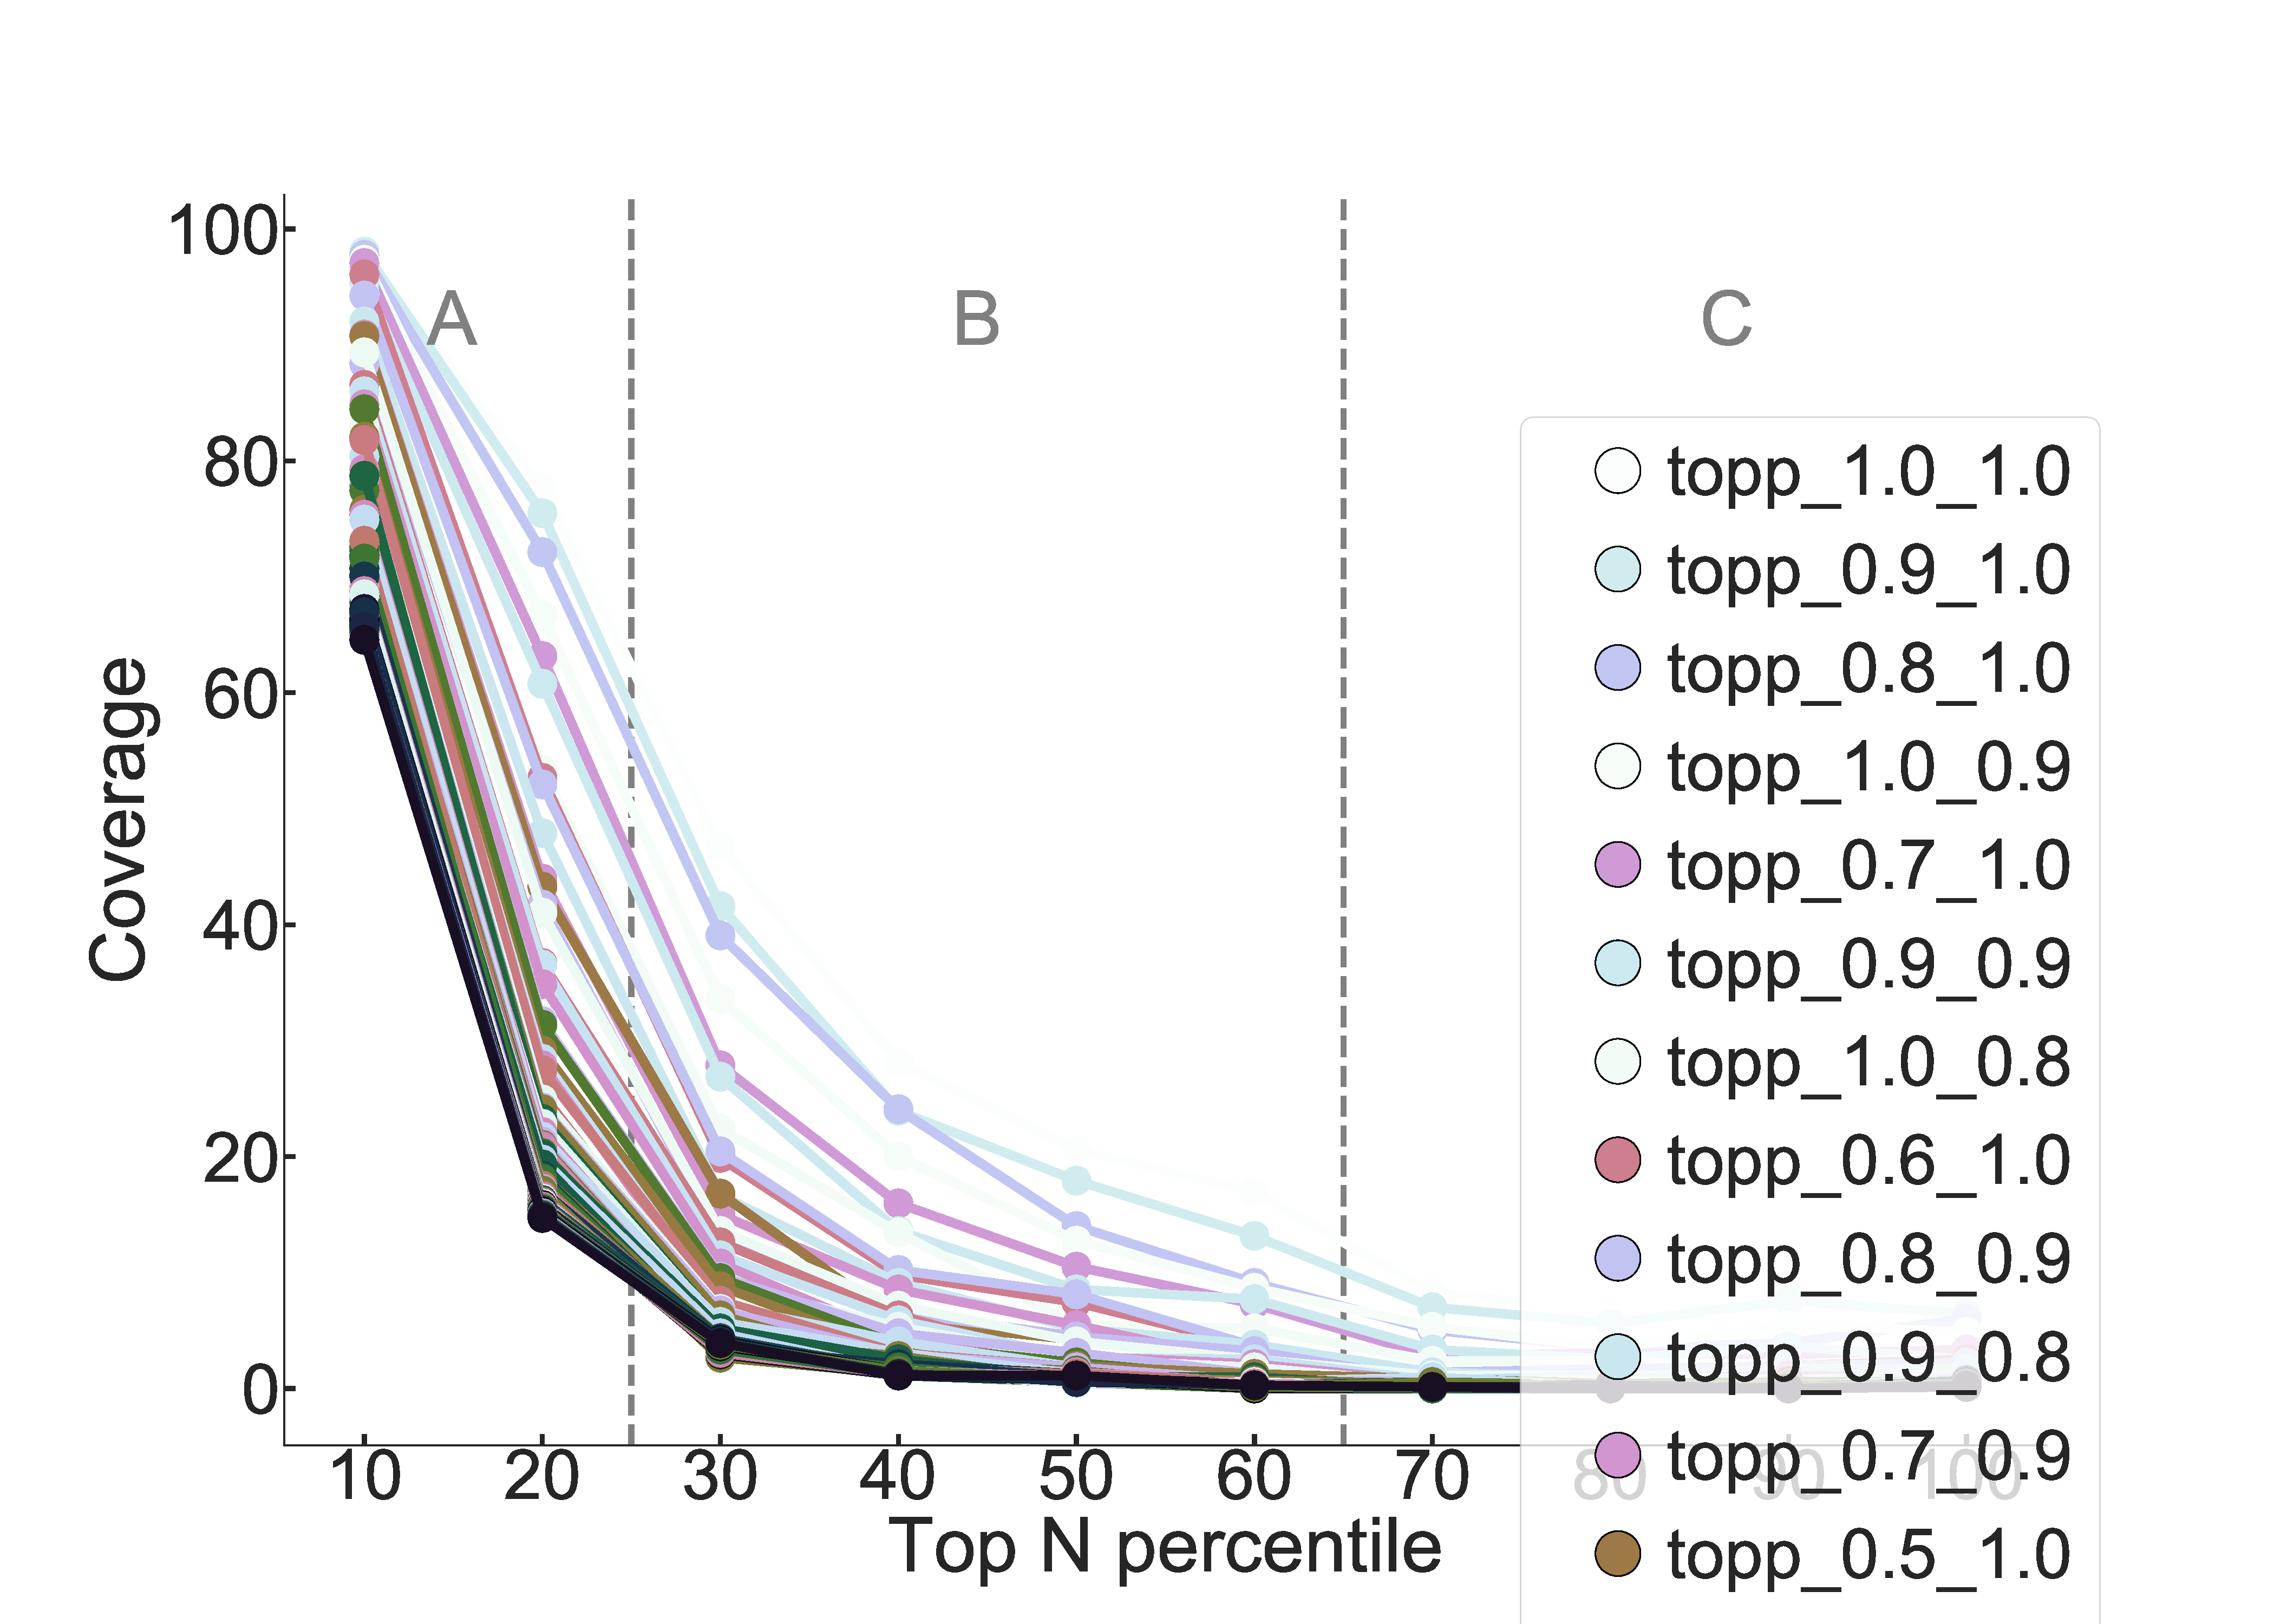
\includegraphics[width=\columnwidth]{figs/percentiles.pdf} \end{figure*}

%\begin{figure*} \centering 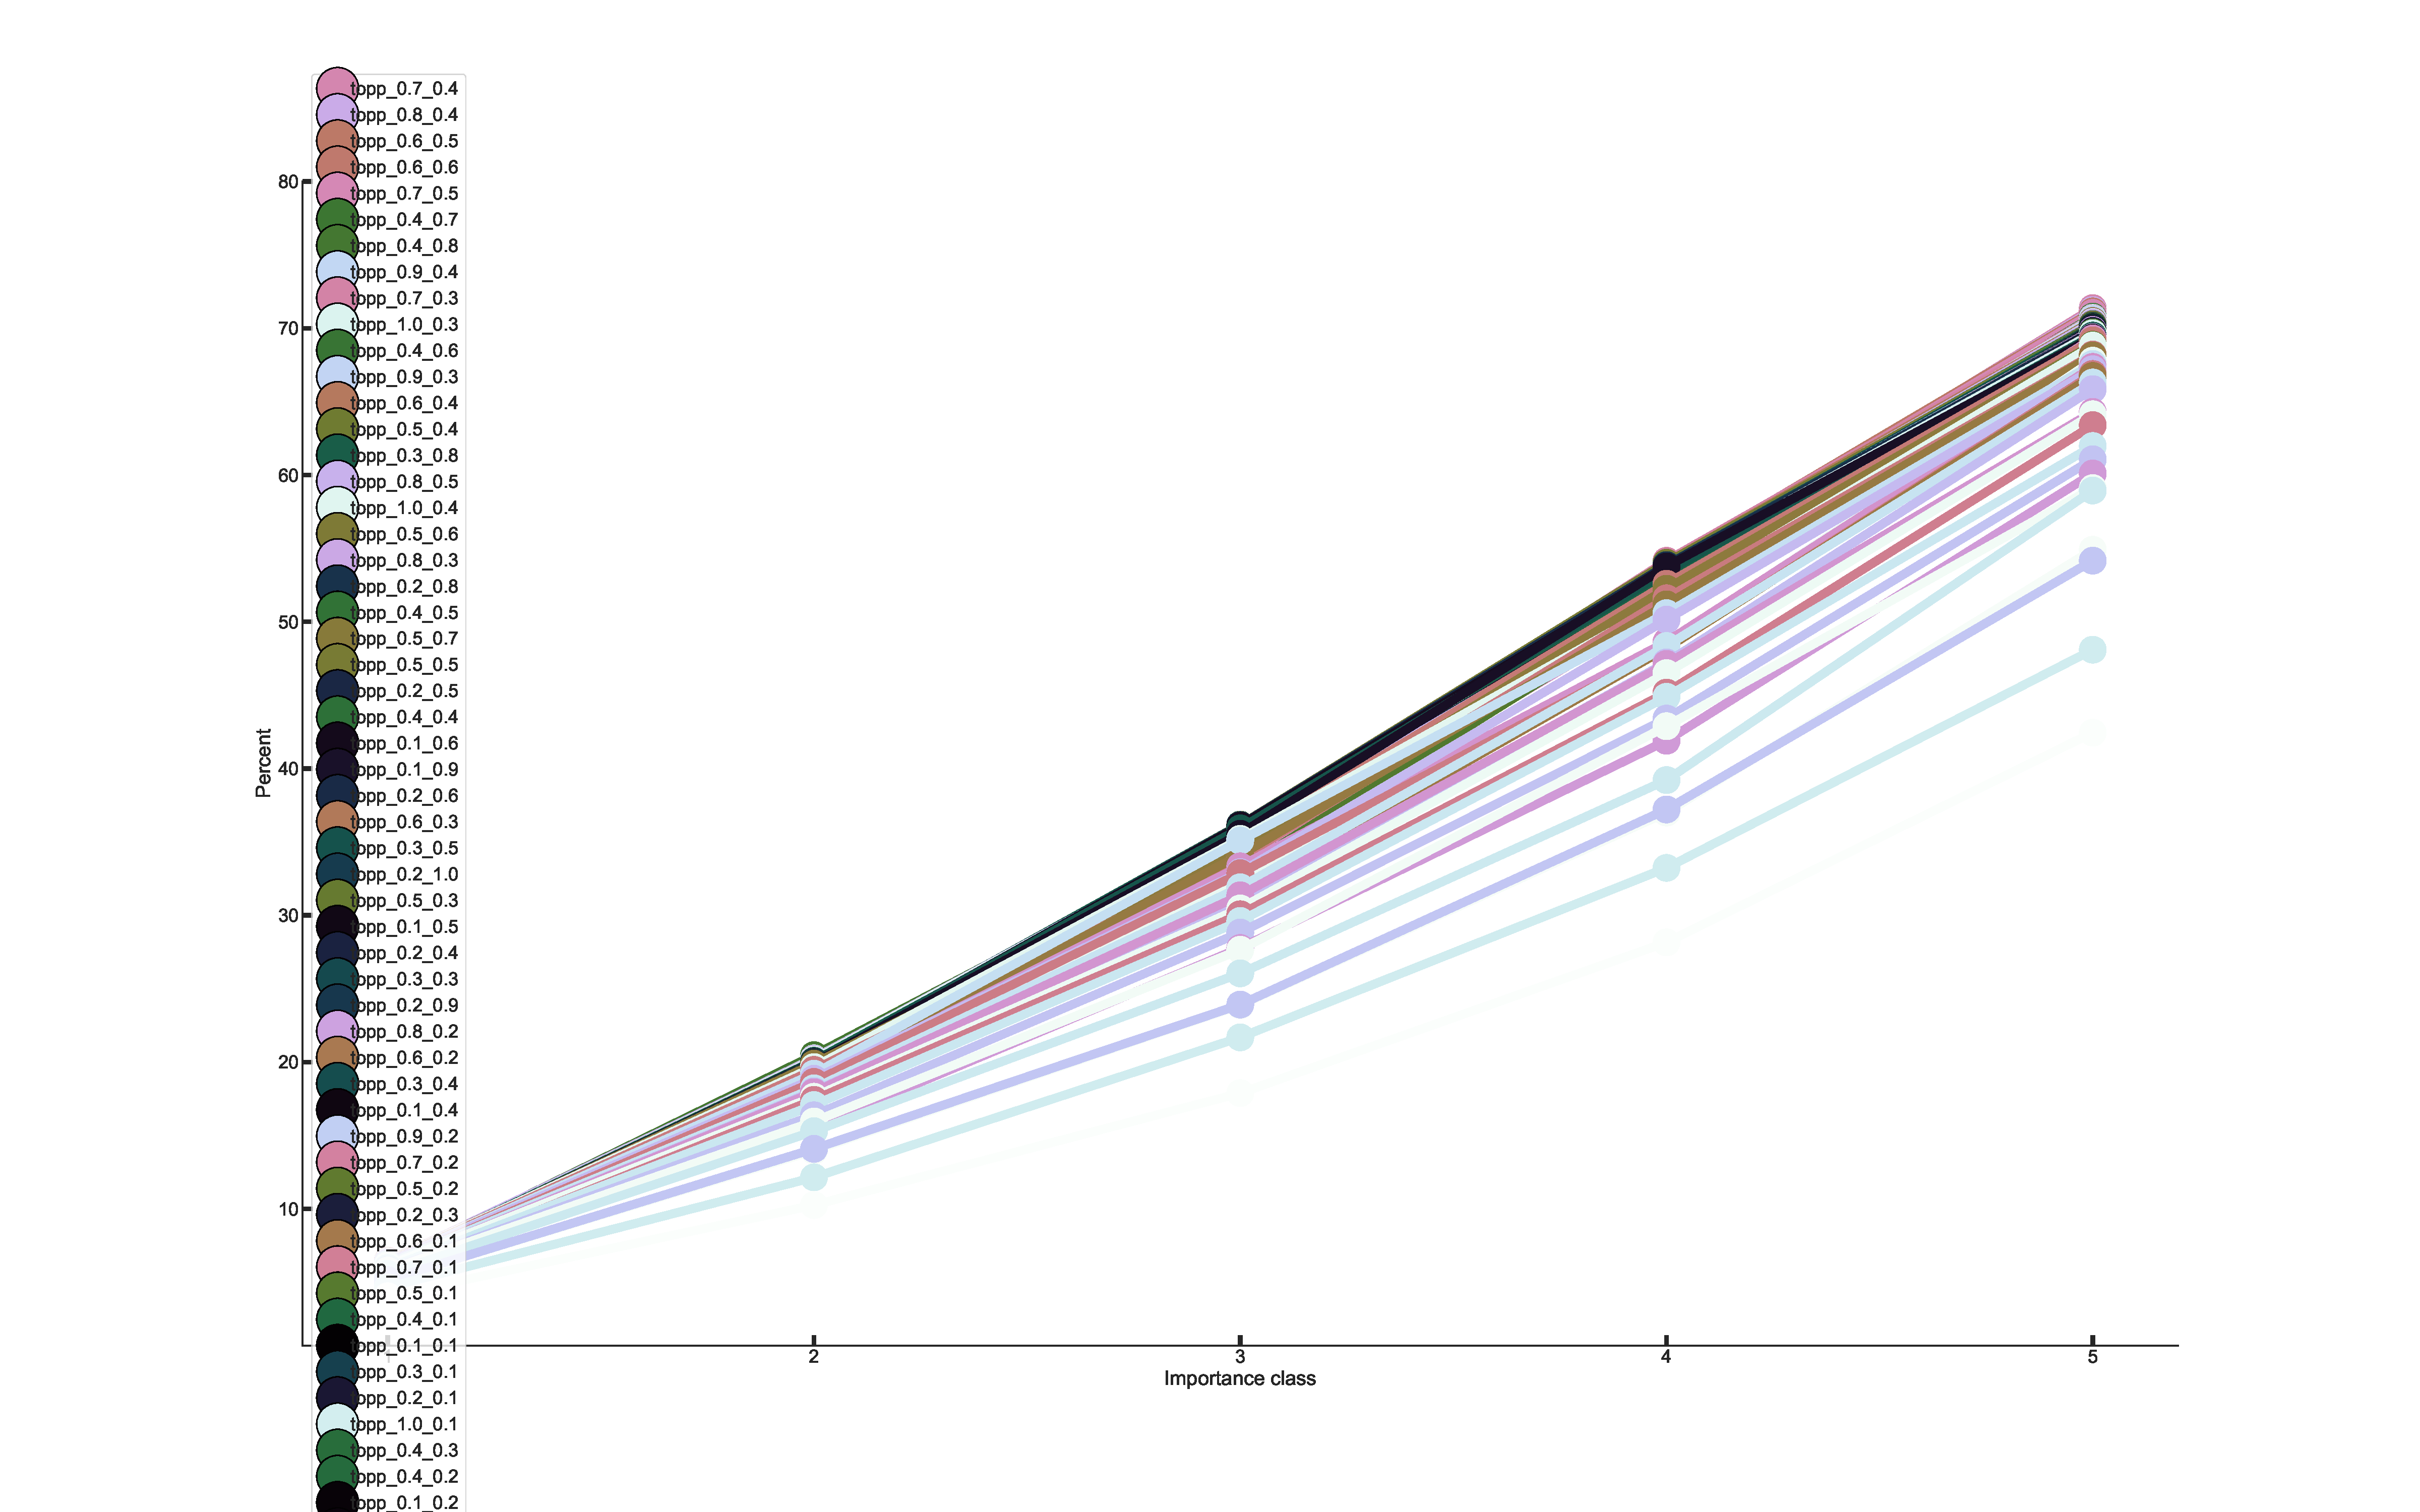
\includegraphics[width=\columnwidth]{figs/local_recall.pdf} \end{figure*}

%\begin{figure*} \centering 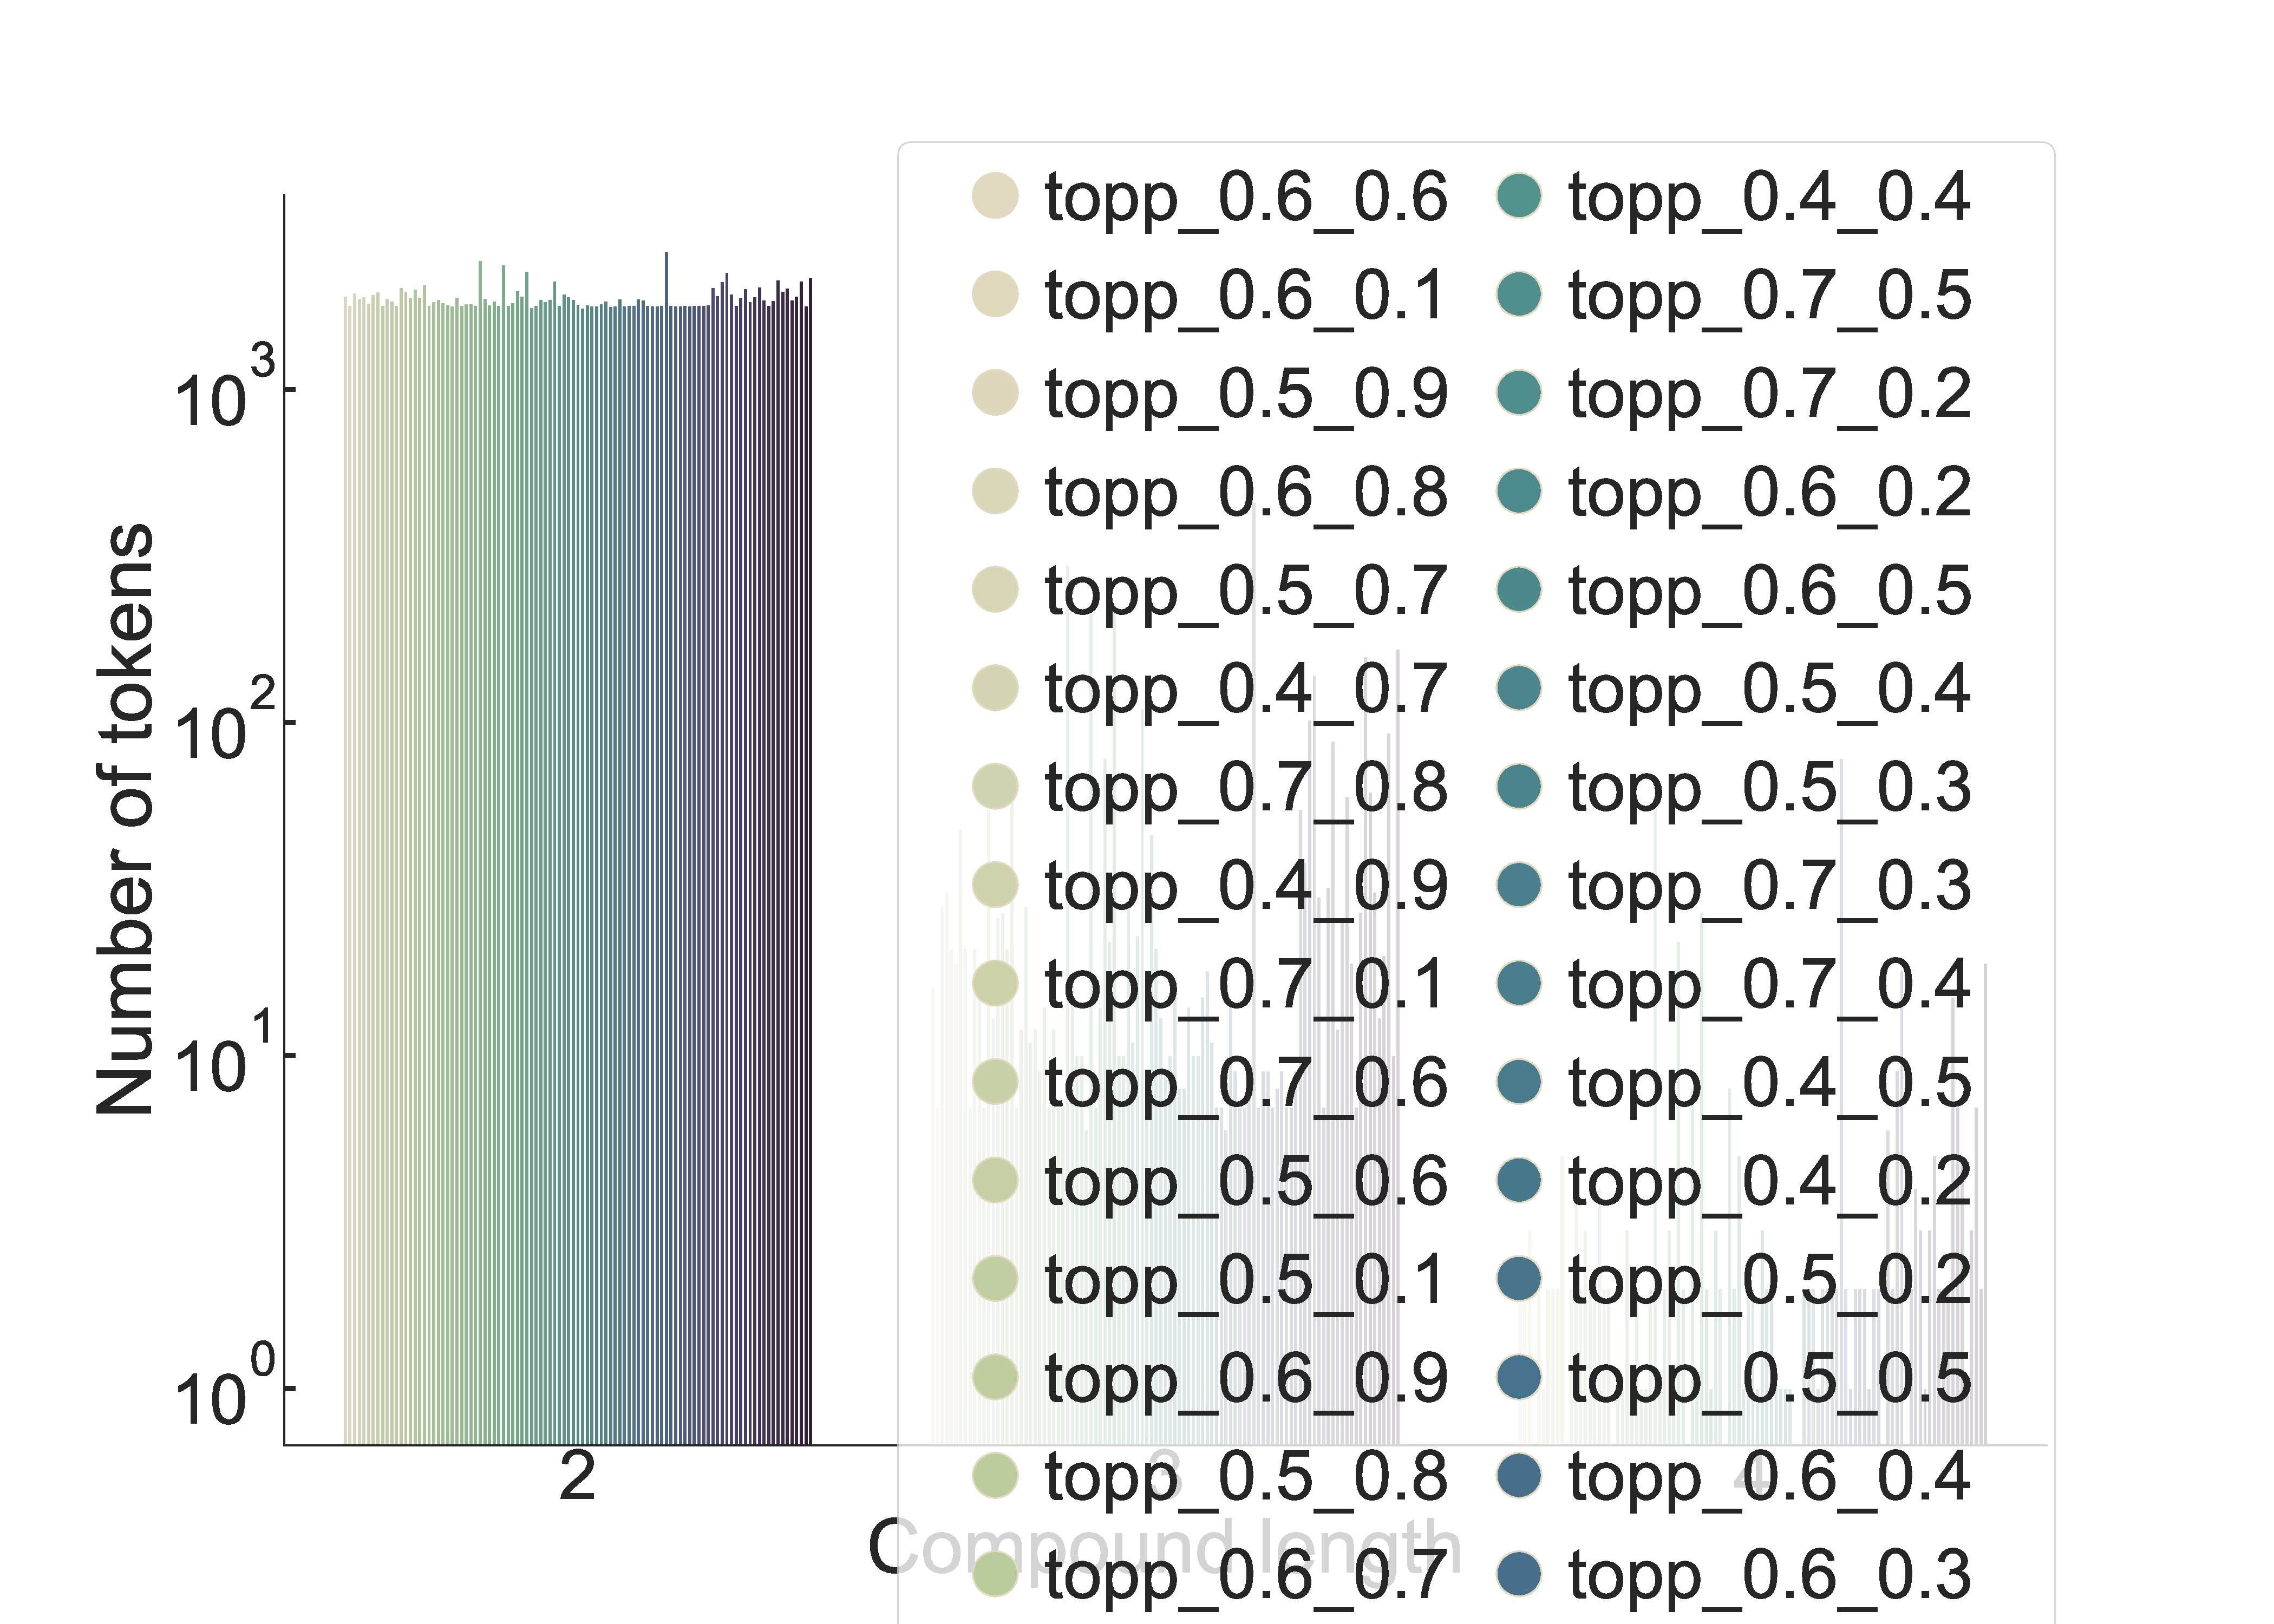
\includegraphics[width=\columnwidth]{figs/compound_lengths.pdf} \end{figure*}


\subsection{Vocabulary}

\begin{itemize}

\item method
	\begin{itemize}
	\item more in-depth analysis of the vocabulary generated by the decoding strategies
	\item types gained / lost in comparison to greedy decoding (or other decoding strategies)
	\item display of the word types generated
	\item out of vocabulary words generated (with respect to the training captions)
	\item average word frequency (with respect to the training captions)
	\item zipf
	\end{itemize}

\item goal
	\begin{itemize}
	\item determine more detailed differences between decoding strategies (not only TTR, novel captions or numbers of types generated)
	\end{itemize}

\item results
	\begin{itemize}
	\item
	\end{itemize}

\end{itemize}

\subsection{Listener Evaluation}

\begin{itemize}

\item method
	\begin{itemize}
	\item evaluate using listener model: for each caption the model tries to distinguish the right target image against a set of similar distractor images (method adopted from \citet{Cohn-Gordon2018})
	\item accuracy or MRR of decisions used to compare the models
	\end{itemize}

\item goal
	\begin{itemize}
	\item check success of pragmatic decoding	
	\item determine whether the increased linguistic diversity in nucleus decoding is used purposefully
	\item see how the non-RSA decoding strategies compare to RSA decoding and to each other
	\end{itemize}

\item results
	\begin{itemize}
	\item best results for RSA decoding
	\item no big differences between other strategies
	\end{itemize}

\end{itemize}

\section{General Discussion}

\begin{itemize}
	\item trainable decoding?
	\item combining decoding strategies (if compatible)
\end{itemize}

\section{Conclusion}



% Bibliography

\bibliographystyle{acl_natbib}
\bibliography{anthology,emnlp2020,literature}

%\appendix

%\section{Appendices}

\end{document}
